% Exemplo de dissertação do INF-UFG com texto em portugues formatado com LaTeX
\documentclass[relatorio, nocolorlinks]{inf-ufg}
% Opções da classe inf-ufg (ao usar mais de uma, separe por vírgulas)
%   [tese]         -> Tese de doutorado.
%   [dissertacao]  -> Dissertação de mestrado (padrão).
%   [monografia]   -> Monografia de especialização.
%   [relatorio]    -> Relatório final de graduação.
%   [abnt]         -> Usa o estilo "abnt-alf" de citação bibliográfica.
%   [nocolorlinks] -> Os links de navegação no texto ficam na cor preta.
% Use esta opção para gerar o arquivo para impressão
%                     da versão final do seu texto!!!

\usepackage{longtable, afterpage, multirow, pdfpages, amsfonts}
%----------------------------------------------------- INICIO DO DOCUMENTO %
\begin{document}
%------------------------------------------ AUTOR, T�TULO E DATA DE DEFESA %
\autor{Fernando Junio Cunha e Sousa}
\autorR{Fernando J. C. Sousa}

\titulo{Análise por Similaridade de Dados Utilizando \textit{Spark}}
%\subtitulo{subtitulo}

\cidade{Goiânia}
\dia{07}
\mes{12}
\ano{2018} % Formato numérico: \dia{01}, \mes{01} e \ano{2009}
%-------------------------------------------------------------- ORIENTADOR %
\orientador{Leonardo Andrade Ribeiro}
\orientadorR{orientadorR}
% Use os comandos a seguir se for Orientadora e nao Orientador.
%\orientadora{Nome da Orientadora}
%\orientadoraR{Nome Reverso da Orientadora}

%\coorientador{Nome do Co-orientador}
%\coorientadorR{Nome Reverso do Co-orientador}
% Use os comandos a seguir se for Co-orientadora e nao Coorientador.
%\coorientadora{Nome da Co-orientadora}
%\coorientadoraR{Nome Reverso da Co-orientadora}

%-------------------------------------------------- INSTITUI��O E PROGRAMA %
\universidade{Universidade Federal de Goiás} % {Universidade Federal de Goiás}
\uni{UFG}         % UFG
\unidade{Instituto de Informática } %Instituto de Informática
%\departamento{Nome do Departamento} %Unidades com mais de um depto.

%\universidadeco{Nome da Universidade do Co-orientador}
%\unico{Sigla da Universidade do Co-orientador}
%\unidadeco{Nome da Unidade Acadêmica do Co-orientador}

%\programa{Nome do Programa de P�s-Gradua��o} % Computa��o
\concentracao{Análise e Processamento de dados, \textit{Big Data}, \textit{Spark Apache}}

%-------------------------------------------------- ELEMENTOS PRÉ-TEXTUAIS %
\capa    % Gera o modelo da capa externa do trabalho%
\publica % Gera a autorização para publicação em formato eletrônico%
\rosto   % Primeira folha interna do trabalho%

 %\begin{figure}[htb]
 % \centering
  %\includegraphics[width=1.20\textwidth]{aprov}
 %\end{figure}

%\includepdf[pages={1}]{aprov.pdf}
 
\begin{aprovacao}
\banca{Dr. Membro da Banca 1}{Instituto de Informática\ -- UFG}
\banca{Dr. Membro da Banca 2}{Instituto de Informática\ -- UFG}
% Use o comando \profa se o membro da banca for do sexo feminino.
\banca{Dr. Membro Externo}{Faculdade de Fora\ -- FF}
\end{aprovacao}
\direitos{Graduou-se em Sistemas de Informação na UFG - Universidade Federal de Goiás. Durante sua graduação, foi monitor na disciplinas de Matemática Discreta no Instituto de Informática.}


\begin{dedicatoria}
\textless Dedicatória do trabalho a alguma pessoa, entidade, etc.\textgreater
\end{dedicatoria}
\begin{agradecimentos}
\textless Texto com agradecimentos àquelas pessoas/entidades que, na opinião do autor, deram alguma contribuição relevante para o desenvolvimento do trabalho.\textgreater
\end{agradecimentos}



\epigrafe{\textless Epígrafe é uma citação relacionada com o tópico do texto\textgreater}
{\textless Nome do autor da citação\textgreater}
{\textless Título da referência à qual a citação pertence\textgreater}

\chaves{\textless Palavra chave 1, palavra chave 2, etc.\textgreater}

\begin{resumo} 
Resumo do trabalho
\end{resumo}


\keys{\textless Keyword 1, keyword 2, etc.\textgreater}

\begin{abstract}{\textless Work title\textgreater}
A sketchy summary of the main points of the text.
\end{abstract}


\tabelas[figtabalg]
%Opções:
%nada [] -> Gera apenas o sumário
%fig     -> Gera o sumário e a lista de figuras
%tab     -> Sumário e lista de tabelas
%alg     -> Sumário e lista de algoritmos
%cod     -> Sumário e lista de códigos de programas
%
% Pode-se usar qualquer combina��o dessas op��es.
% Por exemplo:
%  figtab       -> Sum�rio e listas de figuras e tabelas
%  figtabcod    -> Sum�rio e listas de figuras, tabelas e
%                  c�digos de programas
%  figtabalg    -> Sum�rio e listas de figuras, tabelas e algoritmos
%  figtabalgcod -> Sum�rio e listas de figuras, tabelas, algoritmos e
%                  c�digos de programas

%--------------------------------------------------------------- CAPÌTULOS %
\chapter{Introdução}
\label{cap:intro}
\section{Problema}

Visamos através deste trabalho demonstrar uma dentre várias maneiras para a realização de junção por similaridade de dados. Estas operações de junções por similaridade são essenciais na análise de Big Data \cite{Rong:2017:FS-Join}.

Para a análise de dados provenientes de \textit{Big Data}, a limpeza dos mesmos torna-se uma etapa essencial no processo de preenchimento e manutenção de \textit{Data Warehouses} e repositórios de dados centralizados. Assim sendo, uma das operação de limpeza muito importante é a de agrupar os dados semelhantes com a finalidade de evitar redundâncias nos dados armazenados, e neste processo de juntar é utilizado a operação de junção por similaridade\cite{Chaudhuri:2006:POS:1129754.1129865}.

Faz-se citar o fato de que uma das definições mais aceitas para o termo \textit{Big Data}, é o fato do significar dados muito grandes, muito rápidos ou muito difíceis para que ferramentas existentes possam processar-los\cite{Madden:2012}.

Diante dos fatos acima citados, nosso problema passa pela necessidade de realizar uma junção por similaridade de dados, em dados provenientes de \textit{Big Data}, com a finalidade de realizar a devida higienização dos dados obtidos utilizando da melhor forma possível os recursos computacionais disponíveis.

\section{Objetivo}

Este trabalho objetiva-se em avaliar o \textit{framework} \textit{FS-Join} proposto por \cite{Rong:2017:FS-Join}, utilizando para tal o arcabouço de processamentos distribuídos do \textit{Spark Apache}, e com apoio de implementação da linguagem Scala trabalhando sobre a JVM (\textit{Java Virtual Machine}). 

Utilizando assim o \textit{FS-Join} em parte de dados de \textit{Big Data} e medir sua eficácia em realizar a junção por similaridade dos dados, em relação a tempo de processamento e corretude nos resultados obtidos.

\section{Metodologia de pesquisa}

\section{Estrutura do trabalho}


\chapter{Preliminares}
\label{cap:cap1}

Neste capítulo será realizada uma abordagem a conceitos que não são temas principais deste trabalho, porém, que de alguma forma auxiliam na compreensão e implementação da arquitetura proposta.

Aqui é explorado o conceito de \textit{Big Data} que motivou e originou o problema, ao qual propomos uma solução utilizando o FS-Join. Ainda será encontrada uma abordagem do \textit{framework} \textit{Spark Apache}, realizada uma breve comparação entre o \textit{MapReduce} e ele, buscando explicar os conceitos básicos por trás do \textit{Spark} e realizar uma \textit{overview} sobre as funções utilizadas na implementação. E ainda nesta mesma seção, poderá ser encontrada a motivação para se utilizar a linguagem de programação \textit{Scala}.

\section{\textit{Big Data}}

Não há um consenso entre os autores da área sobre a definição do termo \textit{Big Data} e há um motivo pra isso. Segundo \cite{doi:10.1108/LR-06-2015-0061} o motivo para a não existência uma definição única se deve à rápida evolução da literatura de \textit{Big Data} que impediu o desenvolvimento de uma definição universal e formalmente aceita para o termo.

\textit{Big Data} nasceu com conceito ligado à característica dos dados, que são os \textit{3Vs} -- Volume, Velocidade e Variedade. Passou por conceitos ligados à tecnologia e métodos analíticos necessários para ser fazer o devido uso destes dados. E por conceitos relacionados ao valor que estes dados podem gerar quando há transformação dos dados obtidos em informações, e das informações em valor para o negócio do qual os dados foram obtidos.

Tomaremos neste trabalho a definição de \textit{Big Data} sugerida por \cite{doi:10.1108/LR-06-2015-0061}:  "O \textit{Big Data} é o ativo de informação caracterizado por um volume, velocidade e variedade tão elevados que requer tecnologia específica e métodos analíticos para sua transformação em valor."

Consideramos que volume não está relacionado somente a quantidade de dados gerados ou obtidos através das atividades de \textit{Big Data}, mas também, ao volume de operações necessárias para a higienização dos dados para o devido armazenamento.

\section{Conceitos de operações por similaridade}

Esta seção é destinada à elucidação de conceitos relacionados à operações por similaridade, utilizadas neste trabalho.

\subsection{\textit{Tokenização}}

O processo de \textit{tokenização} é fundamental para aplicações em tarefas de processamento de linguagem natural, como descrito por Bird et al. (2009) \cite{Bird:2009:NLP}, e amplamente utilizado em analises textuais para conversão destes dados em conjuntos de \textit{strings} (do inglês, "cadeia") de caracteres. Estes conjuntos serão compostos por \textit{substrings} (sub-cadeias de caracteres) indivisíveis, ou seja, estes conjuntos serão compostos por partes do texto original na ordem em que aparecem, cada elemento deste conjunto recebe o nome de \textit{token}.  Por este motivo é dado o nome abrasileirado de \textit{tokenização} (no inglês, chamado de \textit{tokenization}).

Para exemplificar o processo de \textit{tokenização}, tomemos cada palavra (no sentido textual) em uma \textit{string} como sendo um \textit{token}, neste contexto, seja "As maquinas irão dominar o mundo." a \textit{string} utilizada como entrada, teremos como saída \{"As","maquinas","irão","dominar","o","mundo."\}. Entretanto aqui o objetivo é utilizar a técnica de \textit{tokenização} para encontrar duplicatas ao comparar duas \textit{strings}, e realizar a \textit{tokenização} em nível tão macro, em que cada \textit{token} corresponda à uma palavra, não será eficiente para verificar caso hajam erros de digitação em apenas um caractere do \textit{token}.

Por este motivo a técnica de \textit{tokenização} utilizada neste trabalho é uma adaptação da técnica de \textit{q-gram} posicional, proposta por Gravano et al. (2001) \cite{Gravano:2001:ASJ:645927.672200}. O processo de criação de \textit{tokens} baseado em \textit{q-grams}, consiste em criar \textit{substrings} deslizando uma janela de comprimento $q$ definida sobre os caracteres das \textit{strings} fornecidas. Com a finalidade de que os caracteres da \textit{string} apareçam exatamente a mesma quantidade de vezes nos \textit{tokens}, são adicionados $q-1$ os novos caracteres  especiais no incio e no fim das \textit{strings}, antes de realizar o processo de \textit{tokenização}. A técnica de \textit{q-gram} posicional, proposta por Gravano et al. (2001) \cite{Gravano:2001:ASJ:645927.672200}, adiciona a cada \textit{token} sua posição na \textit{string} original, neste trabalho sinalizaremos os \textit{tokens} com a ordem de aparição, para o caso de \textit{tokens} iguais porém em posições diferentes, veja mais no exemplo que segue .

Tomemos como \textit{string} de entrada a palavra "amargar" para exemplificar como é realizado o processo neste trabalho, iremos aplicar a \textit{tokenização} fazendo $q=2$, como caractere especial será utilizado "\#", (1) iremos adicionar $q-1$ caracteres especiais no inicio e fim da \textit{string}, portanto, serão adicionados $1$($2-1=1$) caracteres e teremos como saída "\#AMARGAR\#"; (2) o segundo passo é realizar a \textit{tokenização} com temos uma $2-gram$, então, a janela terá comprimento $2$, e portanto como resultado teremos o conjunto \{"\#A1","AM1","MA1","AR1","RG1","GA1","AR2","R\#1"\}. Como há duas ocorrências para o \textit{token} "AR", então, a primeira ocorrência recebe $1$, e a segunda ocorrência recebe $2$, com a finalidade de verificar a posição à título de comparação de duas strings.

Este processo de \textit{tokenização} é fundamental para o processo de junção por similaridade e comparação entre duas \textit{strings}, portanto, fundamental para o bom entendimento e execução da proposta deste trabalho.

\subsection{Junção por similaridade}

No contexto deste trabalho, é necessário entender junção por similaridade como sendo uma operação de comparação entre duas \textit{strings} obtidas à partir de um conjunto de dados de entrada textuais, compara-las com a fim de calcular suas pontuações de similaridade e verificar se suas pontuações não são menores que um determinado valor limite, aqui chamaremos este valor limite de \textit{threshold}, e o representaremos pela letra grega $\theta$(\textit{theta}). Ou seja, dados duas strings $S$ e $V$, aplicadas à uma determinada função de similaridade $sim(S,V)$, dizemos que são similares, caso o resultado dessa função seja maior ou igual à um determinado \textit{threshold}, portanto, são similares caso $sim(S,V) \geq\theta$.

Existem três funções conhecidas para o cálculo da similaridade entre conjuntos, são elas \textit{Jaccard} proposto por Monge et al. (1996)\cite{Monge:1996}[14], \textit{Dice} proposto por Salto et al. 1986\cite{Salton:1986} e Cosseno proposto por Winkler (1999) \cite{Winkler:1999}, cujas definições estão na Tabela \ref{tabelaFuncoesSimilaridade}.

\begin{table}[H]
\centering
 \caption{Funções de Similaridade Baseada em Conjuntos, em que $T$ representa o conjunto de \textit{tokens} de cada \textit{string}}
  \label{tabelaFuncoesSimilaridade}
    \begin{tabular}{|l|c|} 
    \hline Função & Definição \\
    \hline $sim_{jaccard}(S,V)$ & $\dfrac{|T_S \cap T_V|}{|T_S \cup T_V|}$\\ 
    \hline $sim_{dice}(S,V)$ & $\dfrac{2*|T_S \cap T_V|}{|T_S| + |T_V|}$ \\ 
    \hline $sim_{cosseno}(S,V)$ & $\dfrac{|T_S \cap T_V|}{|T_S| * |T_V|}$ \\
    \hline
    \end{tabular}
\end{table}

Neste trabalho é considerado como função de cálculo de similaridade padrão a função \textit{Jaccard}, ou seja, ao referirmos $sim(S,V) \geq\theta$, estamos dizendo que, $sim_{jaccard}(S,V) \geq\theta$.

\section{O \textit{framework Spark Apache}}

Foram consideradas duas ferramentas \textit{open source} para serem utilizadas na elaboração deste trabalho. O \textit{Hadoop} com seu famigerado \textit{MapReduce}, e o Spark com suas \textit{RDDs}, ambas da comunidade Apache. Entretanto, foi selecionado o \textit{framework} \textit{Spark}.

O \textit{framework}\textit{ Spark Apache} possui um arcabouço de ferramentas, e neste trabalho foram utilizadas apenas apenas  as que fornecem a abstração de processamentos paralelos de grandes volumes dados e que podem substituir as primitivas do \textit{MapReduce}.

\textit{MapReduce} e \textit{Spark} são duas estruturas de computação em \textit{cluster}\footnote{\textit{Cluster} é um termo amplamente usado que significa computadores independentes combinados em um sistema unificado por meio de \textit{software} e rede. No nível mais fundamental, quando dois ou mais computadores são usados juntos para resolver um problema, ele é considerado um \textit{cluster}. Os \textit{clusters} geralmente são usados para alta disponibilidade (\textit{HA - High Availability}) para maior confiabilidade ou alta performance computacional (\textit{HPC -  High Performance Computing}) para fornecer maior poder computacional do que um único computador pode fornecer.\cite{1401797-Cluster}} livre, populares para análise de dados em larga escala. Ambas ferramentas ocultam a complexidade na realização de processamentos paralelos e da tolerância a falhas, expondo aos usuários uma \textit{API} (\textit{Application Programming Interface} - em tradução livre "Interface de Programação de Aplicativos") de programação simples. 

Em experimentos realizados em \cite{MpReVsSpark}, o processamento de dados foi explorado de várias formas, com a finalidade de comparar as duas ferramentas. No qual comprovaram que o \textit{MapReduce} possui maior eficácia que o \textit{Spark} em operações de ordenação do tipo \textit{Sort}, e \cite{MpReVsSpark} atribuem isso ao fato de que o \textit{Spark} utiliza clusterização dos dados processados, trabalhando em nós de processamentos em memória, enquanto o \textit{MapReduce} utiliza-se muito de processamentos utilizando o disco. Se faz necessário observar que essa diferença pode ser reduzida dependendo do tipo de disco que será utilizado.

\subsection{\textit{Dataset}}

Antes de descrever do que se trata um \textit{RDD}, é conveniente entender o \textit{dataset} segundo a documentação do \textit{Spark}\cite{SparkPage}. O \textit{dataset} é uma coleção de objetos de domínio específico, fortemente tipada  e podem ser paralelizados utilizando operações funcionais ou relacionais. Cada \textit{dataset} possui uma visão não tipada chamada \textit{DataFrame}, que é o conjunto de dados de uma \textit{Row}. A \textit{Row} representa um vetor com o resultado de um operador contendo um ou mais valores, aceitando valores de tipos diferentes, sejam eles do tipo chave/valor, ou vários valores, por exemplo, $\textit{Row}1(valor1,valor2,valor3)$, onde os valores podem ser acessados pelo índice da posição, aonde o índice 0 corresponde ao valor1 (${Row}1[0]=valor1$), o índice 1 corresponde ao valor2  (${Row}1[1]=valor2$) e assim por diante.

Há operações disponíveis nos \textit{Datasets}, estão dividas entre ações e transformações. Transformações agem sobre o \textit{Dataset} e geram um novo \textit{Dataset}, enquanto ações acionam operações computacionais sobre os \textit{datasets} e retornam os resultados. São exemplos de transformações:  mapear (\textit{map}), filtrar (\textit{filter}), selecionar (\textit{select}) e agregar (\textit{groupBy}). E são exemplos de ação: contadores (\textit{count}), mostrar os dados (\textit{show}), ou gravando dados em arquivos de sistemas.

Este conceito de \textit{dataset} auxilia no melhor entendimento do \textit{RDD} que será discutido na seção à seguir.

\subsection{\textit{RDD} - \textit{Resilient Distributed Dataset}}

Entenda \textit{RDD (Resilient Distributed Dataset)} como um conjunto de dados resilientes e distribuídos, que nada mais é do que uma abstração de memória distribuída, fornecendo aos programadores a possibilidade de executar cálculos em memória de grandes \textit{clusters} de maneira tolerante a falhas.  

A origem dos \textit{RDDs} foi motivada por aplicações que lidam de forma ineficiente com algorítimos interativos e ferramentas interativas para mineração de dados. E que segundo \cite{Zaharia:2012:RDD} , em ambos os casos, o desempenho de manter dados em memória pode melhorar o desempenho em uma ordem de grandeza. 

A tolerância a falhas é eficiente, pois, os \textit{RDDs} fornecem memória compartilhada de forma restrita, ou seja, com base em transformações \textit{coarse-grained} (de alta granularidade), em vez de atualizações \textit{fine-grained} (de baixa granularidade) para o estado compartilhado dos \textit{datasets}. Para deixar a comparação visualmente mais simples, tomemos como exemplo um \textit{dataset} com um milhão de linhas, para este caso uma operação \textit{fine-grained} seria aplicada no menor conjunto possível, no caso uma linha, enquanto que, em uma operação \textit{coarse-grained} seria aplicada sobre o \textit{dataset} como um todo.

No entanto, \cite{Zaharia:2012:RDD} mostra que os \textit{RDDs} são expressivos o suficiente para capturar uma ampla classe de cálculos, incluindo modelos de programação especializados para trabalhos iterativos.

\subsection{Linguagem de Programação \textit{Scala}}

Cabe aqui, descrever o que motivou a escolha da linguagem \textit{Scala} para a realização da implementação do \textit{FS-Join}, mesmo a linguagem não sendo tão popular.

A linguagem \textit{Scala} foi criada em 2001-2004 na \textit{EPFL} (\textit{École Polytechnique Fédérale de Lausanne})  em seu laboratório de métodos de programação, com a finalidade de aprimorar o suporte à linguagens de componentes de \textit{software}. Esses estudos foram orientados principalmente para duas ideias. Primeiro, a linguagem de aplicação do componente deveria ser escalável, ou seja, deveria ser possível usar os mesmos conceitos tanto para escrever pequenas parte de um aplicativo, quanto para escrever grandes partes do mesmo. Os desenvolvedores da linguagem estavam focados implementar de maneira eficiente a abstração, composição, e mecanismos de decomposição, em vez de introduzir um grande número de tipos primitivos, úteis somente em altos níveis de escalabilidade. Em segundo lugar, é bastante natural criar uma linguagem que unifique e generalize orientação a objeto com programação funcional. Uma das principais inovações técnicas da linguagem \textit{Scala} é o conceito que faz a junção entre esses dois paradigmas \cite{Glybovets2010}.

A linguagem \textit{Scala} não fornece primitivas de comunicação e
sincronização para programação paralela. O núcleo da linguagem é construído de forma a simplificar a criação de bibliotecas que suportam vários modelos de paralelismo construídos sobre o modelo atual da linguagem principal \cite{Glybovets2010}.

Existe certa semelhança entre os programas escritos em \textit{Java} e os escritos em \textit{Scala}. Os programas escritos em \textit{Java} podem interagir livremente com os códigos escritos em \textit{Scala} e vice-versa. Programas escritos em \textit{Scala} podem substituir partes críticas de código escritos em \textit{Java}, que exigem alto nível de processamento paralelo ou escrita funcional, e ainda ambos permanecerem dentro do mesmo projeto, pois a linguagem \textit{Scala} roda sobre o \textit{JVM} (\textit{Java Virtual Machine}), da \textit{Oracle}. Havia uma compatibilidade do Scala com o .\textit{NET} \textit{Framework}, da \textit{Microsoft}, e que porém foi descontinuada nas versões mais recentes da linguagem.

Portanto, por se tratar de uma linguagem que fornece boas ferramentas nativas para processamentos paralelos, e por ainda ser nativamente compatível com o \textit{Framework} \textit{Spark Apache}, além de integrar com projetos \textit{Java} pré-existentes, a mesma foi selecionada para integrar o arcabouço de ferramentas utilizadas neste trabalho.

Mais informações sobre a linguagem podem ser obtidas na documentação no site próprio da mesma \cite{ScalaPage}.

\subsection{O \textit{MapReduce}}

Esta seção se faz importante pelo fato que o trabalho \cite{Rong:2017:FS-Join}, no qual se baseia este trabalho, utilizou a arquitetura do \textit{MapReduce} para realizar a implementação do \textit{framework} proposto e este trabalho propõe faze-lo utilizando o \textit{framework} \textit{Spark Apache}. Na próxima seção será descrito o processo análogo para o \textit{Spark Apache}.

Segundo \cite{Rong:2017:FS-Join} o \textit{MapReduce} foi proposto para facilitar o processamento de conjuntos de dados de larga escala em \textit{clusters} não compartilhados, utilizando computadores comerciais não especializados. Por sua escalabilidade e tolerância a falhas, ela se tornou a plataforma de fato para o processamento de \textit{Big Data}.

O \textit{MapReduce} consiste em duas primitivas, \textit{Map} (mapear) e \textit{Reduce} (reduzir). Na estrutura do \textit{MapReduce}, todos os registros são representados como pares chave/valor (\textit{key/value}). O conjunto de dados de entrada geralmente é armazenado em um sistema de arquivos distribuído (\textit{DFS - Distributed File System}), em vários nós de execução da carga de trabalho. Depois que a carga de trabalho  é enviada para o MapReduce, os registros são fornecidos aos nós do mapeador em partes. Cada registro será analisado no par de chaves/valores \textit{<key1, value1>} e é aplicada a função de \textit{Map} que cria uma nova lista com pares de chave/valor \textit{lista(<key2, value2>).} Os pares de chave/valor com a mesma chave serão enviados para o mesmo nó de redução durante a fase de reprodução aleatória e serão agrupados por sua chave na forma de lista de valores \textit{<key2, lista(value2)>}. O redutor receberá a lista de valores \textit{<key2, lista(value2)>} e aplicará a função \textit{Reduce} a eles. Por fim, o redutor produzirá uma lista de pares de chave/valor \textit{lista(<key3, value3>)} e os gravará no sistema de arquivos distribuído. O processo acima pode ser formalizado como abaixo.

\begin{itemize}
\item  Map: $\textit{<key1,value1>} \rightarrow \textit{lista(<key2, value2>)}$;
\item Reduce: $\textit{<key2, lista(value2)>} \rightarrow \textit{lista(<key3, value3>)}$;
\end{itemize}

Nesta seção será discutida as funções do \textit{Spark} utilizadas para substituir as funções no \textit{MapReduce}.   As funções listadas aqui foram obtidas da documentação original do \textit{Spark}\cite{SparkPage}, e apoiado nos exemplos do livro \cite{karau2015learning}.

Em face à primitiva \textit{Map} do \textit{MapReduce} será utilizada a primitiva 

\subsection{Funções do \textit{Spark} utilizadas no projeto}

Esta seção será dedicada a explicar alguns conceitos das operações realizadas pelo \textit{Spark}, realizando um paralelo entre suas operações e as operações do \textit{MapReduce}.

Segundo \cite{LearningSparkAl}, o \textit{Spark} utiliza \textit{RDDs} em seus nós de processamento, e permite que sejam realizadas \textbf{ações} e \textbf{transformações} como operação sobre os \textit{RDDs}.  \textbf{Ações} são operações que retornam um resultado para a aplicação ou armazenam  os dados e realizam um cálculo, \textit{count()} e \textit{first()} são exemplos de ações realizadas sobre os \textit{RDDs}. Já \textbf{transformações} realizadas sobre um determinado \textit{RDD} retorna um novo \textit{RDD}, por exemplo as operações de \textit{map()} e \textit{filter()}.

As operações de \textbf{ação} utilizadas no projeto são:
\begin{itemize}
\item \textit{\textbf{count}}: Operação que contabiliza a quantidade de elementos em um \textit{RDD}, geralmente a quantidade de linhas.ido em um \textit{RDD}.
\item \textit{\textbf{first}}: Retorna o primeiro elemento contido em um \textit{RDD}.
\item \textit{\textbf{reduce}}: Utiliza uma função que opera sobre dois elementos do mesmo tipo no \textit{RDD} e retorna um novo elemento do mesmo tipo. Por exemplo, para somar todos os elementos inteiros de um \textit{RDD}, podemos utilizar a função soma (+) dos inteiros, e obteremos como resultado um único valor inteiro correspondente à soma de todos elementos do \textit{RDD}. Pode ser utilizada em alguns casos como substituta da função de mesmo nome do \textit{MapReduce}, porém, a função mais adequada do \textit{Spark} em vários casos será a \textit{reduceByKey}.
\end{itemize}
As operações de \textbf{transformação} utilizadas no projeto são:
\begin{itemize}
\item \textit{\textbf{map}}: Esta operação tem como propósito aplicar uma determinada função em cada um dos elementos de um \textit{RDD} e retornar um novo \textit{RDD} contendo o resultado da função aplicada. Será utilizada ainda como substituta de função homônima no \textit{MapReduce}.
\item \textit{\textbf{flatMap}}: Semelhante ao \textit{map}, porém, cada item de entrada pode ser mapeado para zero ou mais itens de saída, portanto, a função deve retornar uma sequência de elementos em vez de um único item, geralmente utilizada para iterar nos elementos de uma lista que estão em uma única linha de um \textit{RDD} e retornar um elemento por linha do \textit{RDD}.
\item \textit{\textbf{mapPartition}}: Semelhante ao \textit{map}, mas é executado separadamente em cada partição (bloco) do RDD.
\item \textit{\textbf{reduceByKey}}: Utilizada quando os objetos contidos no \textit{RDD} são do tipo chave/valor, no qual os objetos que possuem mesma chave serão agrupados, e será aplicada a ação \textit{reduce}, utilizando uma função, sobre os valores que possuem chaves iguais. É elegível como substituta da função \textit{reduce} do \textit{MapReduce} em muitos casos.
\item \textit{\textbf{groupByKey}}: Possui funcionalidade próxima à função \textit{reduceByKey}, agrupando os valores baseados nas chaves em comum, porém, neste caso gera uma lista contendo os valores que possuem mesma chave agrupando por chave, não permitindo que sejam aplicadas funções sobre os valores. É elegível como substituta da função \textit{reduce} do \textit{MapReduce} dependendo da necessidade.
\item \textbf{\textit{aggregateByKey}}: Possui funcionalidade próxima à \textit{groupByKey}, porém quando chamado em um conjunto de dados de pares chave/valor, retorna um conjunto de dados de pares em que os valores de cada chave são agregados usando as funções combinadas fornecidas e um valor inicial neutro, nulo ou uma lista vazia. Permite tipos valores agregados que são diferente do tipo do valor contido nos pare, evitando alocações desnecessárias.
\item \textbf{\textit{filter}}: Retornar um novo conjunto de dados formado por elementos selecionados do \textit{RDD} origem em que passarem por uma função de verificação cujo retorno seja verdadeiro quando aplicada ao elemento.
\item \textbf{\textit{sortByKey}}: Aplicada aos \textit{RDDs} que contenham pares do tipo chave/valor, e retorna um novo \textit{RDD} que possua elementos ordenados pela chave do par, permitindo que seja selecionado se as chaves serão ordenadas em ordem crescente, ou decrescente.
\end{itemize}

As funções citadas acima são as mais utilizadas na implementação proposta do algorítimo, e foram expostas com a finalidade de facilitar a leitura, e entendimento do algorítimo implementado.











\chapter{Trabalhos relacionados}
\label{cap:trab_rel}

Existem muitos estudos sobre algoritmos de junção de similaridade de \textit{strings} em memória \cite{Gravano:2001:ASJ:645927.672200}, \cite{Sarawagi:2004:ESJ:1007568.1007652},\cite{Chaudhuri:2006:POS:1129754.1129865}, \cite{Arasu:2006:EES:1182635.1164206}, \cite{Bayardo:2007:SUP:1242572.1242591}, \cite{Xiao:2008:ESJ:1367497.1367516}, que podem ser categorizados em dois tipos: junção por similaridade de sequência baseada em conjunto (\textit{SSJoin}) e junção por similaridade de sequência baseada em caracteres (\textit{EDJoin}).  O \textit{SSJoin} considera a sequência como um conjunto de símbolos e utiliza funções de similaridade baseadas em conjuntos, como \textit{Jaccard}, \textit{Dice} e \textit{Cosseno}, como uma sequência de caracteres e utiliza a distância de edição como sua função de similaridade. Este trabalho concentra-se no \textit{SSJoin}.

Para responder eficientemente às associações de similaridade de \textit{strings}, a maioria dos trabalhos existentes segue uma estrutura de filtro e verificação \cite{Li:2008:EMF:1546682.1547171}, \cite{Wang:2012:WBP:2213836.2213847}, \cite{Rong:2013:6319300}, \cite{Li:2015:ESJ:2723372.2723733}. No estágio de filtro, os pares de \textit{strings} diferentes são removidos com base em alguns métodos de filtragem eficientes, por exemplo, utilizando filtro de prefixo, e assim os candidatos são gerados. Na fase de verificação, os candidatos são verificados calculando-se a pontuação de similaridade exata. Mais precisamente, o trabalho de Chaudhri et al. (2016)\cite{Chaudhuri:2006:POS:1129754.1129865} propôs o método de filtragem de prefixo utilizando \textit{tokens} de prefixo como assinaturas. A proposta feita por Xiao et al. (2008)\cite{Xiao:2008:ESJ:1367497.1367516} melhorou o filtro de prefixo, integrando a informação de posição e informação de comprimento. Bayardo et al. (2007) \cite{Bayardo:2007:SUP:1242572.1242591} construiu índices invertidos para todas as \textit{strings}, onde as chaves são \textit{tokens} das assinaturas e os valores são as \textit{strings} correspondentes contendo os \textit{tokens}. Li at al (2018)\cite{Li:2008:EMF:1546682.1547171}, Xiao et al. (2008)\cite{Xiao:2008:ESJ:1367497.1367516} propuseram outras técnicas de otimização para a lista invertida. No trabalho de Wang at al (2012)\cite{Wang:2012:WBP:2213836.2213847} estenderam a filtragem de prefixo baseada em comprimento fixo e propuseram uma filtragem de prefixo de tamanho variável. Para a mesma \textit{string}, Wang et al. (2012)\cite{Wang:2012:WBP:2213836.2213847} extrai mais \textit{tokens} do que os métodos de filtragem de prefixo baseados em comprimento fixo e constrói múltiplos índices invertidos de forma incremental. No trabalho de Wang at al (2012)\cite{Wang:2012:WBP:2213836.2213847} exploraram vários tipos de ordens globais e propuseram um algoritmo baseado em filtragem de múltiplos prefixos. Os vários filtros de prefixo são aplicados de forma incremental. No trabalho de Li at al (2015)\cite{Li:2015:ESJ:2723372.2723733} projetaram um índice baseado em árvore para prefixos de múltiplos atributos e propuseram um modelo de custo para guiar a construção do índice. Diferente desses estudos, neste trabalho focamos em como oferecer suporte a junções de similaridade em grande escala utilizando o \textit{Spark Apache}.

Para suportar junções de similaridade de strings em \textit{big data}, muitas contribuições recentes foram direcionadas à implementação de algoritmos em \textit{MapReduce} \cite{Vernica:2010:EPS:1807167.1807222}, \cite{Metwally:2012}, \cite{Deng:2014}. Mais precisamente, Vernica at al (2010) \cite{Vernica:2010:EPS:1807167.1807222} propôs um algoritmo baseado em assinatura, chamado \textit{RIDPairsPPJoin}, que segue a estrutura de filtro e verificação. Na fase de filtro, ele cria assinaturas para cada sequência, selecionando um conjunto de \textit{tokens} como prefixo, no qual os \textit{tokens} de uma \textit{string} são ordenados de acordo com uma ordem global pré-definida. Cada \textit{token} do prefixo é considerado como uma chave e uma \textit{string} com a chave inclusa é considerada como seu valor correspondente. As \textit{strings} com as mesmas assinaturas são transmitidas à um grupo para verificação adicional. Na fase de verificação, um índice invertido para cada grupo de \textit{strings} é criado para acelerar o processamento, e os métodos de filtragem são aplicados para podar ainda mais os pares dissimilares. No entanto, \textit{RIDPairsPPJoin} possui duas limitações: 
(1) uma sequência de strings pode ser duplicada várias vezes, uma vez que vários \textit{tokens} são selecionados como assinaturas, que incorrem em alto custo de ordenação e cálculos redundantes; e (2) os valores em cada \textit{job} do \textit{Reduce} são strings contendo a mesma chave, que possuem tamanhos diferentes. Portanto, não há garantia de balanceamento de carga nos nós \textit{Reduce}. Em Metwally et al. (2012)\cite{Metwally:2012} é relatado que \textit{RIPPJoin} não é escalável.

Em Metwally et al. (2012)\cite{Metwally:2012} propuseram um novo algoritmo \textit{V-Smart-Join} para junções por semelhança em \textit{multisets} e vetores. \textit{V-Smart-Join} por forma junções por similaridades em duas fases: \textbf{junção} e \textbf{similaridade}. Na fase de \textbf{junção}, ele contém vários \textit{jobs} e o \textit{MapReduce} fornece implementações diferentes, incluindo o \textit{Online-Aggregation}, pesquisa e distribuição. Na fase de \textbf{similaridade}, os resultados parciais são agregados para obter os pares de candidatos finais. De acordo com Metwally et al. (2012)\cite{Metwally:2012}, o \textit{Online-Aggregation} tem a melhor escalabilidade entre as três implementações. Na fase de junção, cada \textit{token} das strings é enviado como uma chave. Isto é como construir um índice invertido para todos os \textit{tokens} no conjunto de dados no \textit{HDFS}. \textit{V-Smart-Join} possui os mesmos problemas (duplicações e problemas de balanceamento de carga) como \textit{RIDPairsPPJoin}. Além disso, possui duas limitações extras: (1) o custo de enumerar cada par de corridas em cada lista invertida é dispendioso; e (2) nenhuma filtragem é aplicada durante o processo de junção, o que resulta em um alto número de falsos positivos, custo extra de ordenação e computação desnecessária.

Em Deng et al. (2014)\cite{Deng:2014} propuseram um método de junção de similaridade, chamado \textit{MassJoin}, para strings longas baseado em seu algoritmo centralizado por proposto em \cite{Li:2011}. No trabalho de Deng et al. (2014)\cite{Deng:2014}, cada \textit{string} \(s\) em \(S\) é particionada para segmentos pares e todos eles como suas assinaturas; para cada \textit{string} \(t\) em \(T\), ele deve gerar muitas assinaturas para assegurar que haja uma assinatura comum com $s$ que com comprimento em $\ceil{|t|*\theta} \leq |s| \leq \floor{|t|/\theta}$. Se $\theta = 0,8$ e $| t | = 100$, o intervalo de comprimento é $[80,125]$. Então, para cada inteiro de \(80\) à \(125\), a \textit{string} $t$ irá gerar assinaturas separadamente. Porém, possui ainda os mesmos problemas que o \textit{RIDPairsPPJoin}.

Para resolver os problemas de duplicação e balanceamento de carga, Rong et al. (2017)\cite{Rong:2017:FS-Join} propõe um novo \textit{framework} para junção por similaridade, chamado de \textit{FS-Join}. O \textit{FS-Join} aplica um método de particionamento vertical para particionar cada \textit{string} em segmentos disjuntos. Em que todos os segmentos em uma mesma partição constituem um fragmento. Os fragmentos possuem tamanhos iguais (ou similares). Na fase \textit{Map}, o \textit{FS-Join} utiliza os \textit{IDs} de partição como chaves e os segmentos correspondentes como valores. Como os segmentos são disjuntos, então, não há duplicações. Além disso, na fase \textit{Reduce}, todos os segmentos pertencentes ao mesmo fragmento são ordenados em um mesmo nó \textit{Reduce}. Como os fragmentos possuem os mesmos tamanhos, o \textit{FS-Join} garante um balanceamento de carga adequado. 
%A Tabela I resume a comparação de FS-Join e os métodos do estado da técnica, isto é, \textit{RIDPairsPPJoin} proposto por Vernica et al (2010)\cite{Vernica:2010:EPS:1807167.1807222}, \textit{V-Smart-Join} proposto por Metwally et al (2012)\cite{Metwally:2012} e \textit{MassJoin} proposto por Deng et al (2014)\cite{Deng:2014}, fornecida em Rong et al(2017)\cite{Rong:2017:FS-Join}.

Este trabalho propõe reproduzir o \textit{framework} \textit{FS-Join} proposto por \cite{Rong:2017:FS-Join}, aplicando todas as melhorias sugeridas. Respeitando as fases propostas, porém, utilizando como \textit{framework} para processamento paralelo e distribuído o \textit{Apache Spark} como substituto do utilizado por Rong et al. (2017)\cite{Rong:2017:FS-Join}.

\chapter{O \textit{FS-Join}}
\label{cap:cap2}

Este capítulo é destinado à apresentação do framework proposto no trabalho de Rong et al. (2017)\cite{Rong:2017:FS-Join}. Aqui é exposto a arquitetura do \textit{FS-Join} proposta por Rong et al. (2017) \cite{Rong:2017:FS-Join}, com as devidas adequações às tecnologias utilizadas neste trabalho, são discutidos o particionamento vertical, os filtros propostos por Rong et al. (2017)\cite{Rong:2017:FS-Join}, e será apresentado o algoritmo do \textit{FS-Join} tal como foi implementado. Neste trabalho não foi considerado o que Rong et al. (2017)\cite{Rong:2017:FS-Join} chama de particionamento horizontal.

\section{A arquitetura do \textit{FS-Join}}

A arquitetura do \textit{FS-Join} proposta por  Rong et al. (2017) \cite{Rong:2017:FS-Join} pode ser particionada em três etapas: Ordenação, Filtragem e Verificação. Cada um dessas etapas serão exploradas à seguir, ressaltando que, este trabalho preservou a arquitetura original e serão descritas como são realizadas as operações utilizando o \textit{Spark}, enquanto no trabalho original utiliza-se o \textit{MapReduce}, como destacado no capítulo anterior.

\subsection{Ordenação}

Nesta etapa será ordenada toda coleção de caracteres recebidos como entrada. Então, o primeiro passo a ser executado no \textit{FS-Join} é realizar uma ordenação global dos dados recebidos, essa ordenação sera representada por $O$. O método de ordenação utilizado por \cite{Rong:2017:FS-Join} é dividido em duas fases, sendo elas:
\begin{enumerate}
\item  Calcular a frequência para cada \textit{token};
\item  Classificar os \textit{tokens} em ordem crescente tomando como parâmetro de ordenação a frequência do \textit{token}.
\end{enumerate}

O algoritmo que calcula a frequência para a ordenação global do\textit{ FS-Join} utiliza funções do \textit{Spark} para calcular a frequência e obter a ordem global da coleção de \textit{strings} que estão em um \textit{RDD} recebidos como entrada.

\subsection{Filtragem}

Nesta etapa o \textit{FS-Join} utiliza uma função do \textit{Spark} para gerar pares de \textit{strings} candidatos removendo os pares dissimilares sem calcular necessariamente calcular os valores precisos de similaridade.  Segundo \cite{Rong:2017:FS-Join} esta é a operação principal do \textit{FS-Join} é composta por duas fases, que serão descritas à seguir, sendo elas: fase de particionamento e fase de junção. 

Na fase de particionamento, é recebido como entrada o \textit{RDD} contendo as \textit{strings} originais e os \textit{tokens} em ordenação global $O$, obtidas na etapa anterior, e seleciona um número de \textit{pivôs} a partir de $O$ (mais detalhes nas próximas seções). Em seguida, ordena os {tokens} nas \textit{strings} recebidas de acordo com a a ordem global $O$ e particiona cada uma das \textit{strings} em vários \textit{segmentos} utilizando cada um dos \textit{pivôs} que foram cuidadosamente selecionados.  os \textit{tokens} em cada sequência recebida de acordo com a ordem global, cada sequência em vários segmentos com base em um conjunto de \textit{pivôs} cuidadosamente escolhidos (mais detalhes nas próximas seções). 

Após todas essas fases, o \textit{FS-Join} irá tratar o \textit{ID}\footnote{ID - Identificador do objeto gerado, que pode ser um número ou um \textit{token}} da partição como chave,  e o valor correspondente como valor, ao enviar para função \textit{Map}.  Os segmentos pertencentes à mesma partição serão ordenados no mesmo nó de redução. Em cada redutor, o \textit{gerador de chaves candidatas} do \textit{FS-Join} gera candidatos usando um índice invertido baseado em prefixo e vários métodos de filtragem, por exemplo, filtragem por comprimento, filtragem com reconhecimento de \textit{segmento} (veja a próxima seção). A saída do $i$-ésimo redutor é uma lista de pares $(p, c)$, onde $p = (s, t)$ é um par de strings, enquanto $c$ é o número de \textit{tokens} comuns entre $s$ e $t$ na $i$-ésima partição, ou seja, o $i$-ésimo segmento de $s$ e $t$.

\subsection{Verificação}

Durante a etapa de verificação, que é a ultima etapa executada pelo \textit{FS-Join} irá utilizar uma função do \textit{Spark}  para verificar os \textit{candidatos} gerados na fase de filtro anterior. Se o número final de \textit{tokens} comuns de um par de strings for maior que um \textit{threshold}\footnote{\textit{Threshold} - valor limite} $\sigma$, então é uma resposta aceita. Caso contrário, não é. Os detalhes serão discutidos nas próximas seções.
\begin{figure}[ht]
\centering
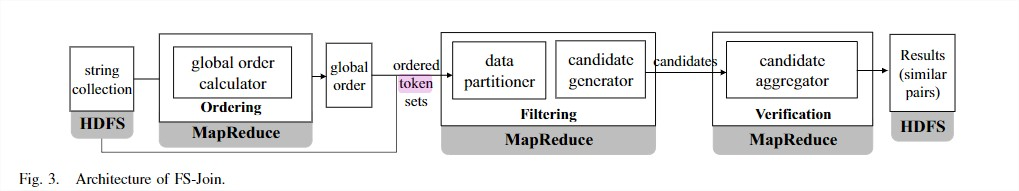
\includegraphics[scale=0.4]{fig/arqFSJoin.jpg}
\caption{Arquitetura do \textit{FS-Join}}
\end{figure}

\section{Particionamento Vertical}



\section{O Algoritmo do \textit{FS-Join}}

%\input{./tabelas/similarCalc}
\begin{algorithm2e}[H]
\DontPrintSemicolon % Some LaTeX compilers require you to use \dontprintsemicolon instead
\Entrada{Uma coleção de conjuntos C; um \emph{threshold} $\theta$}
\Saida{Um conjunto D que contêm todos os pares $(x_1, x_2)$, em que $sim(x_1, x_2) \ge \gamma$}
$I_1, I_2, \dots I_u \gets \emptyset$ \;
$D \gets \emptyset$ \; 
\For{$x_1 \in C$ }{
  $M \gets $ um mapa vazio do conjunto, id e ps (ps = pontuação de sobreposição)\;
  $M(id, ps) \gets \emptyset$ \;
  \For{$t \in$ maxprefix$(x_1)$}{ \;
    Remove todos $x_2 \in I_t$, em que $|x_2| < $ minsize$(x_1)$ \;
    \For{$x_2 \in I_t$}{ \;
        M$(x_2) \gets$ (M$(x_2)$.ps + 1) \;
        \If{}{ \;
        }
    }
  }

  $i \gets i + 1$\; 
}
\Return{location};
\caption{Algoritmo FS-Join}
\label{algo:duplicate}
\end{algorithm2e}


\chapter{Experimentos (Sugestões baseadas no artigo)}
\label{cap:cap3}

\section{Configuração de experimentos}
\section{Escalabilidade}
\section{Efeito da seleção de pivô}
\section{Efeito dos métodos de associação}
\section{Efeito das otimizações}


\chapter{Conclusão}
\label{cap:conclusoes}
%------------------------------------------------------------ BIBLIOGRAFIA %
\cleardoublepage
%\nocite{*} %%% Retire esta linha para gerar a bibliografia com apenas as
           %%% refer�ncias usadas no seu texto!
\arial
%\bibliography{./bib/modelo-tese} %%% Nomes dos seus arquivos .bib
\bibliography{./bib/ref} %%% Nomes dos seus arquivos .bib
\label{ref-bib}

%--------------------------------------------------------------- AP�NDICES %
%\apendices

%\chapter{Exemplo de um Ap�ndice}
\label{apend:1}
Ap�ndicess s�o iniciados com o comando \verb|\apendices|.
Ap�ndicess s�o iniciados com o comando \verb|\apendices|.
Ap�ndicess s�o iniciados com o comando \verb|\apendices|.
Ap�ndicess s�o iniciados com o comando \verb|\apendices|.
Ap�ndicess s�o iniciados com o comando \verb|\apendices|.
Ap�ndicess s�o iniciados com o comando \verb|\apendices|.
Ap�ndicess s�o iniciados com o comando \verb|\apendices|.
Ap�ndicess s�o iniciados com o comando \verb|\apendices|.
Ap�ndicess s�o iniciados com o comando \verb|\apendices|.
Ap�ndicess s�o iniciados com o comando \verb|\apendices|.
Ap�ndicess s�o iniciados com o comando \verb|\apendices|.
Ap�ndicess s�o iniciados com o comando \verb|\apendices|.
Ap�ndicess s�o iniciados com o comando \verb|\apendices|.
Ap�ndicess s�o iniciados com o comando \verb|\apendices|.
Ap�ndicess s�o iniciados com o comando \verb|\apendices|.
Ap�ndicess s�o iniciados com o comando \verb|\apendices|.

Ap�ndicess s�o iniciados com o comando \verb|\apendices|.
Ap�ndicess s�o iniciados com o comando \verb|\apendices|.
Ap�ndicess s�o iniciados com o comando \verb|\apendices|.
Ap�ndicess s�o iniciados com o comando \verb|\apendices|.
Ap�ndicess s�o iniciados com o comando \verb|\apendices|.
Ap�ndicess s�o iniciados com o comando \verb|\apendices|.
Ap�ndicess s�o iniciados com o comando \verb|\apendices|.
Ap�ndicess s�o iniciados com o comando \verb|\apendices|.
Ap�ndicess s�o iniciados com o comando \verb|\apendices|.
Ap�ndicess s�o iniciados com o comando \verb|\apendices|.
Ap�ndicess s�o iniciados com o comando \verb|\apendices|.
Ap�ndicess s�o iniciados com o comando \verb|\apendices|.

Ap�ndicess s�o iniciados com o comando \verb|\apendices|.
Ap�ndicess s�o iniciados com o comando \verb|\apendices|.
Ap�ndicess s�o iniciados com o comando \verb|\apendices|.
Ap�ndicess s�o iniciados com o comando \verb|\apendices|.
Ap�ndicess s�o iniciados com o comando \verb|\apendices|.
Ap�ndicess s�o iniciados com o comando \verb|\apendices|.
Ap�ndicess s�o iniciados com o comando \verb|\apendices|.
Ap�ndicess s�o iniciados com o comando \verb|\apendices|.
Ap�ndicess s�o iniciados com o comando \verb|\apendices|.
Ap�ndicess s�o iniciados com o comando \verb|\apendices|.
Ap�ndicess s�o iniciados com o comando \verb|\apendices|.
Ap�ndicess s�o iniciados com o comando \verb|\apendices|.
Ap�ndicess s�o iniciados com o comando \verb|\apendices|.
Ap�ndicess s�o iniciados com o comando \verb|\apendices|.

Ap�ndicess s�o iniciados com o comando \verb|\apendices|.
Ap�ndicess s�o iniciados com o comando \verb|\apendices|.
Ap�ndicess s�o iniciados com o comando \verb|\apendices|.
Ap�ndicess s�o iniciados com o comando \verb|\apendices|.
Ap�ndicess s�o iniciados com o comando \verb|\apendices|.
Ap�ndicess s�o iniciados com o comando \verb|\apendices|.
Ap�ndicess s�o iniciados com o comando \verb|\apendices|.
Ap�ndicess s�o iniciados com o comando \verb|\apendices|.
Ap�ndicess s�o iniciados com o comando \verb|\apendices|.
Ap�ndicess s�o iniciados com o comando \verb|\apendices|.
Ap�ndicess s�o iniciados com o comando \verb|\apendices|.
Ap�ndicess s�o iniciados com o comando \verb|\apendices|.
Ap�ndicess s�o iniciados com o comando \verb|\apendices|.
Ap�ndicess s�o iniciados com o comando \verb|\apendices|.

Ap�ndicess s�o iniciados com o comando \verb|\apendices|.
Ap�ndicess s�o iniciados com o comando \verb|\apendices|.
Ap�ndicess s�o iniciados com o comando \verb|\apendices|.
Ap�ndicess s�o iniciados com o comando \verb|\apendices|.
Ap�ndicess s�o iniciados com o comando \verb|\apendices|.
Ap�ndicess s�o iniciados com o comando \verb|\apendices|.
Ap�ndicess s�o iniciados com o comando \verb|\apendices|.
Ap�ndicess s�o iniciados com o comando \verb|\apendices|.
Ap�ndicess s�o iniciados com o comando \verb|\apendices|.
Ap�ndicess s�o iniciados com o comando \verb|\apendices|.
Ap�ndicess s�o iniciados com o comando \verb|\apendices|.
Ap�ndicess s�o iniciados com o comando \verb|\apendices|.
Ap�ndicess s�o iniciados com o comando \verb|\apendices|.
Ap�ndicess s�o iniciados com o comando \verb|\apendices|.

Ap�ndicess s�o iniciados com o comando \verb|\apendices|.
Ap�ndicess s�o iniciados com o comando \verb|\apendices|.
Ap�ndicess s�o iniciados com o comando \verb|\apendices|.
Ap�ndicess s�o iniciados com o comando \verb|\apendices|.
Ap�ndicess s�o iniciados com o comando \verb|\apendices|.
Ap�ndicess s�o iniciados com o comando \verb|\apendices|.
Ap�ndicess s�o iniciados com o comando \verb|\apendices|.
Ap�ndicess s�o iniciados com o comando \verb|\apendices|.
Ap�ndicess s�o iniciados com o comando \verb|\apendices|.
Ap�ndicess s�o iniciados com o comando \verb|\apendices|.
Ap�ndicess s�o iniciados com o comando \verb|\apendices|.
Ap�ndicess s�o iniciados com o comando \verb|\apendices|.
Ap�ndicess s�o iniciados com o comando \verb|\apendices|.
Ap�ndicess s�o iniciados com o comando \verb|\apendices|.

Ap�ndicess s�o iniciados com o comando \verb|\apendices|.
Ap�ndicess s�o iniciados com o comando \verb|\apendices|.
Ap�ndicess s�o iniciados com o comando \verb|\apendices|.
Ap�ndicess s�o iniciados com o comando \verb|\apendices|.
Ap�ndicess s�o iniciados com o comando \verb|\apendices|.
Ap�ndicess s�o iniciados com o comando \verb|\apendices|.
Ap�ndicess s�o iniciados com o comando \verb|\apendices|.
Ap�ndicess s�o iniciados com o comando \verb|\apendices|.
Ap�ndicess s�o iniciados com o comando \verb|\apendices|.
Ap�ndicess s�o iniciados com o comando \verb|\apendices|.
Ap�ndicess s�o iniciados com o comando \verb|\apendices|.
Ap�ndicess s�o iniciados com o comando \verb|\apendices|.
Ap�ndicess s�o iniciados com o comando \verb|\apendices|.
Ap�ndicess s�o iniciados com o comando \verb|\apendices|.

Ap�ndicess s�o iniciados com o comando \verb|\apendices|.
Ap�ndicess s�o iniciados com o comando \verb|\apendices|.
Ap�ndicess s�o iniciados com o comando \verb|\apendices|.
Ap�ndicess s�o iniciados com o comando \verb|\apendices|.
Ap�ndicess s�o iniciados com o comando \verb|\apendices|.
Ap�ndicess s�o iniciados com o comando \verb|\apendices|.
Ap�ndicess s�o iniciados com o comando \verb|\apendices|.
Ap�ndicess s�o iniciados com o comando \verb|\apendices|.
Ap�ndicess s�o iniciados com o comando \verb|\apendices|.
Ap�ndicess s�o iniciados com o comando \verb|\apendices|.
Ap�ndicess s�o iniciados com o comando \verb|\apendices|.
Ap�ndicess s�o iniciados com o comando \verb|\apendices|.
Ap�ndicess s�o iniciados com o comando \verb|\apendices|.
Ap�ndicess s�o iniciados com o comando \verb|\apendices|.

Ap�ndicess s�o iniciados com o comando \verb|\apendices|.
Ap�ndicess s�o iniciados com o comando \verb|\apendices|.
Ap�ndicess s�o iniciados com o comando \verb|\apendices|.
Ap�ndicess s�o iniciados com o comando \verb|\apendices|.
Ap�ndicess s�o iniciados com o comando \verb|\apendices|.
Ap�ndicess s�o iniciados com o comando \verb|\apendices|.
Ap�ndicess s�o iniciados com o comando \verb|\apendices|.
Ap�ndicess s�o iniciados com o comando \verb|\apendices|.
Ap�ndicess s�o iniciados com o comando \verb|\apendices|.
Ap�ndicess s�o iniciados com o comando \verb|\apendices|.
Ap�ndicess s�o iniciados com o comando \verb|\apendices|.
Ap�ndicess s�o iniciados com o comando \verb|\apendices|.
Ap�ndicess s�o iniciados com o comando \verb|\apendices|.
Ap�ndicess s�o iniciados com o comando \verb|\apendices|.

Ap�ndicess s�o iniciados com o comando \verb|\apendices|.
Ap�ndicess s�o iniciados com o comando \verb|\apendices|.
Ap�ndicess s�o iniciados com o comando \verb|\apendices|.
Ap�ndicess s�o iniciados com o comando \verb|\apendices|.
Ap�ndicess s�o iniciados com o comando \verb|\apendices|.
Ap�ndicess s�o iniciados com o comando \verb|\apendices|.
Ap�ndicess s�o iniciados com o comando \verb|\apendices|.
Ap�ndicess s�o iniciados com o comando \verb|\apendices|.
Ap�ndicess s�o iniciados com o comando \verb|\apendices|.
Ap�ndicess s�o iniciados com o comando \verb|\apendices|.
Ap�ndicess s�o iniciados com o comando \verb|\apendices|.
Ap�ndicess s�o iniciados com o comando \verb|\apendices|.
Ap�ndicess s�o iniciados com o comando \verb|\apendices|.
Ap�ndicess s�o iniciados com o comando \verb|\apendices|.

Ap�ndicess s�o iniciados com o comando \verb|\apendices|.
Ap�ndicess s�o iniciados com o comando \verb|\apendices|.
Ap�ndicess s�o iniciados com o comando \verb|\apendices|.
Ap�ndicess s�o iniciados com o comando \verb|\apendices|.
Ap�ndicess s�o iniciados com o comando \verb|\apendices|.
Ap�ndicess s�o iniciados com o comando \verb|\apendices|.
Ap�ndicess s�o iniciados com o comando \verb|\apendices|.
Ap�ndicess s�o iniciados com o comando \verb|\apendices|.
Ap�ndicess s�o iniciados com o comando \verb|\apendices|.
Ap�ndicess s�o iniciados com o comando \verb|\apendices|.
Ap�ndicess s�o iniciados com o comando \verb|\apendices|.
Ap�ndicess s�o iniciados com o comando \verb|\apendices|.
Ap�ndicess s�o iniciados com o comando \verb|\apendices|.
Ap�ndicess s�o iniciados com o comando \verb|\apendices|.

Ap�ndicess s�o iniciados com o comando \verb|\apendices|.
Ap�ndicess s�o iniciados com o comando \verb|\apendices|.
Ap�ndicess s�o iniciados com o comando \verb|\apendices|.
Ap�ndicess s�o iniciados com o comando \verb|\apendices|.
Ap�ndicess s�o iniciados com o comando \verb|\apendices|.
Ap�ndicess s�o iniciados com o comando \verb|\apendices|.
Ap�ndicess s�o iniciados com o comando \verb|\apendices|.
Ap�ndicess s�o iniciados com o comando \verb|\apendices|.
Ap�ndicess s�o iniciados com o comando \verb|\apendices|.
Ap�ndicess s�o iniciados com o comando \verb|\apendices|.
Ap�ndicess s�o iniciados com o comando \verb|\apendices|.
Ap�ndicess s�o iniciados com o comando \verb|\apendices|.
Ap�ndicess s�o iniciados com o comando \verb|\apendices|.
Ap�ndicess s�o iniciados com o comando \verb|\apendices|.

Ap�ndicess s�o iniciados com o comando \verb|\apendices|.
Ap�ndicess s�o iniciados com o comando \verb|\apendices|.
Ap�ndicess s�o iniciados com o comando \verb|\apendices|.
Ap�ndicess s�o iniciados com o comando \verb|\apendices|.
Ap�ndicess s�o iniciados com o comando \verb|\apendices|.
Ap�ndicess s�o iniciados com o comando \verb|\apendices|.
Ap�ndicess s�o iniciados com o comando \verb|\apendices|.
Ap�ndicess s�o iniciados com o comando \verb|\apendices|.
Ap�ndicess s�o iniciados com o comando \verb|\apendices|.
Ap�ndicess s�o iniciados com o comando \verb|\apendices|.
Ap�ndicess s�o iniciados com o comando \verb|\apendices|.
Ap�ndicess s�o iniciados com o comando \verb|\apendices|.
Ap�ndicess s�o iniciados com o comando \verb|\apendices|.
Ap�ndicess s�o iniciados com o comando \verb|\apendices|.

Ap�ndicess s�o iniciados com o comando \verb|\apendices|.
Ap�ndicess s�o iniciados com o comando \verb|\apendices|.
Ap�ndicess s�o iniciados com o comando \verb|\apendices|.
Ap�ndicess s�o iniciados com o comando \verb|\apendices|.
Ap�ndicess s�o iniciados com o comando \verb|\apendices|.
Ap�ndicess s�o iniciados com o comando \verb|\apendices|.
Ap�ndicess s�o iniciados com o comando \verb|\apendices|.
Ap�ndicess s�o iniciados com o comando \verb|\apendices|.
Ap�ndicess s�o iniciados com o comando \verb|\apendices|.
Ap�ndicess s�o iniciados com o comando \verb|\apendices|.
Ap�ndicess s�o iniciados com o comando \verb|\apendices|.
Ap�ndicess s�o iniciados com o comando \verb|\apendices|.
Ap�ndicess s�o iniciados com o comando \verb|\apendices|.
Ap�ndicess s�o iniciados com o comando \verb|\apendices|.

%\chapter{Exemplo de Outro Ap�ndice}
\label{apend:2}
Texto do Ap�ndice~\ref{apend:2}.

Ap�ndices s�o iniciados com o comando \verb|\apendices|.
Ap�ndices s�o iniciados com o comando \verb|\apendices|.
Ap�ndices s�o iniciados com o comando \verb|\apendices|.
Ap�ndices s�o iniciados com o comando \verb|\apendices|.
Ap�ndices s�o iniciados com o comando \verb|\apendices|.
Ap�ndices s�o iniciados com o comando \verb|\apendices|.
Ap�ndices s�o iniciados com o comando \verb|\apendices|.
Ap�ndices s�o iniciados com o comando \verb|\apendices|.
Ap�ndices s�o iniciados com o comando \verb|\apendices|.
Ap�ndices s�o iniciados com o comando \verb|\apendices|.
Ap�ndices s�o iniciados com o comando \verb|\apendices|.
Ap�ndices s�o iniciados com o comando \verb|\apendices|.
Ap�ndices s�o iniciados com o comando \verb|\apendices|.
Ap�ndices s�o iniciados com o comando \verb|\apendices|.
Ap�ndices s�o iniciados com o comando \verb|\apendices|.
Ap�ndices s�o iniciados com o comando \verb|\apendices|.

Ap�ndices s�o iniciados com o comando \verb|\apendices|.
Ap�ndices s�o iniciados com o comando \verb|\apendices|.
Ap�ndices s�o iniciados com o comando \verb|\apendices|.
Ap�ndices s�o iniciados com o comando \verb|\apendices|.
Ap�ndices s�o iniciados com o comando \verb|\apendices|.
Ap�ndices s�o iniciados com o comando \verb|\apendices|.
Ap�ndices s�o iniciados com o comando \verb|\apendices|.
Ap�ndices s�o iniciados com o comando \verb|\apendices|.
Ap�ndices s�o iniciados com o comando \verb|\apendices|.
Ap�ndices s�o iniciados com o comando \verb|\apendices|.
Ap�ndices s�o iniciados com o comando \verb|\apendices|.
Ap�ndices s�o iniciados com o comando \verb|\apendices|.

Ap�ndices s�o iniciados com o comando \verb|\apendices|.
Ap�ndices s�o iniciados com o comando \verb|\apendices|.
Ap�ndices s�o iniciados com o comando \verb|\apendices|.
Ap�ndices s�o iniciados com o comando \verb|\apendices|.
Ap�ndices s�o iniciados com o comando \verb|\apendices|.
Ap�ndices s�o iniciados com o comando \verb|\apendices|.
Ap�ndices s�o iniciados com o comando \verb|\apendices|.
Ap�ndices s�o iniciados com o comando \verb|\apendices|.
Ap�ndices s�o iniciados com o comando \verb|\apendices|.
Ap�ndices s�o iniciados com o comando \verb|\apendices|.
Ap�ndices s�o iniciados com o comando \verb|\apendices|.
Ap�ndices s�o iniciados com o comando \verb|\apendices|.
Ap�ndices s�o iniciados com o comando \verb|\apendices|.
Ap�ndices s�o iniciados com o comando \verb|\apendices|.

Ap�ndices s�o iniciados com o comando \verb|\apendices|.
Ap�ndices s�o iniciados com o comando \verb|\apendices|.
Ap�ndices s�o iniciados com o comando \verb|\apendices|.
Ap�ndices s�o iniciados com o comando \verb|\apendices|.
Ap�ndices s�o iniciados com o comando \verb|\apendices|.
Ap�ndices s�o iniciados com o comando \verb|\apendices|.
Ap�ndices s�o iniciados com o comando \verb|\apendices|.
Ap�ndices s�o iniciados com o comando \verb|\apendices|.
Ap�ndices s�o iniciados com o comando \verb|\apendices|.
Ap�ndices s�o iniciados com o comando \verb|\apendices|.
Ap�ndices s�o iniciados com o comando \verb|\apendices|.
Ap�ndices s�o iniciados com o comando \verb|\apendices|.
Ap�ndices s�o iniciados com o comando \verb|\apendices|.
Ap�ndices s�o iniciados com o comando \verb|\apendices|.

Ap�ndices s�o iniciados com o comando \verb|\apendices|.
Ap�ndices s�o iniciados com o comando \verb|\apendices|.
Ap�ndices s�o iniciados com o comando \verb|\apendices|.
Ap�ndices s�o iniciados com o comando \verb|\apendices|.
Ap�ndices s�o iniciados com o comando \verb|\apendices|.
Ap�ndices s�o iniciados com o comando \verb|\apendices|.
Ap�ndices s�o iniciados com o comando \verb|\apendices|.
Ap�ndices s�o iniciados com o comando \verb|\apendices|.
Ap�ndices s�o iniciados com o comando \verb|\apendices|.
Ap�ndices s�o iniciados com o comando \verb|\apendices|.
Ap�ndices s�o iniciados com o comando \verb|\apendices|.
Ap�ndices s�o iniciados com o comando \verb|\apendices|.
Ap�ndices s�o iniciados com o comando \verb|\apendices|.
Ap�ndices s�o iniciados com o comando \verb|\apendices|.

Ap�ndices s�o iniciados com o comando \verb|\apendices|.
Ap�ndices s�o iniciados com o comando \verb|\apendices|.
Ap�ndices s�o iniciados com o comando \verb|\apendices|.
Ap�ndices s�o iniciados com o comando \verb|\apendices|.
Ap�ndices s�o iniciados com o comando \verb|\apendices|.
Ap�ndices s�o iniciados com o comando \verb|\apendices|.
Ap�ndices s�o iniciados com o comando \verb|\apendices|.
Ap�ndices s�o iniciados com o comando \verb|\apendices|.
Ap�ndices s�o iniciados com o comando \verb|\apendices|.
Ap�ndices s�o iniciados com o comando \verb|\apendices|.
Ap�ndices s�o iniciados com o comando \verb|\apendices|.
Ap�ndices s�o iniciados com o comando \verb|\apendices|.
Ap�ndices s�o iniciados com o comando \verb|\apendices|.
Ap�ndices s�o iniciados com o comando \verb|\apendices|.

Ap�ndices s�o iniciados com o comando \verb|\apendices|.
Ap�ndices s�o iniciados com o comando \verb|\apendices|.
Ap�ndices s�o iniciados com o comando \verb|\apendices|.
Ap�ndices s�o iniciados com o comando \verb|\apendices|.
Ap�ndices s�o iniciados com o comando \verb|\apendices|.
Ap�ndices s�o iniciados com o comando \verb|\apendices|.
Ap�ndices s�o iniciados com o comando \verb|\apendices|.
Ap�ndices s�o iniciados com o comando \verb|\apendices|.
Ap�ndices s�o iniciados com o comando \verb|\apendices|.
Ap�ndices s�o iniciados com o comando \verb|\apendices|.
Ap�ndices s�o iniciados com o comando \verb|\apendices|.
Ap�ndices s�o iniciados com o comando \verb|\apendices|.
Ap�ndices s�o iniciados com o comando \verb|\apendices|.
Ap�ndices s�o iniciados com o comando \verb|\apendices|.

Ap�ndices s�o iniciados com o comando \verb|\apendices|.
Ap�ndices s�o iniciados com o comando \verb|\apendices|.
Ap�ndices s�o iniciados com o comando \verb|\apendices|.
Ap�ndices s�o iniciados com o comando \verb|\apendices|.
Ap�ndices s�o iniciados com o comando \verb|\apendices|.
Ap�ndices s�o iniciados com o comando \verb|\apendices|.
Ap�ndices s�o iniciados com o comando \verb|\apendices|.
Ap�ndices s�o iniciados com o comando \verb|\apendices|.
Ap�ndices s�o iniciados com o comando \verb|\apendices|.
Ap�ndices s�o iniciados com o comando \verb|\apendices|.
Ap�ndices s�o iniciados com o comando \verb|\apendices|.
Ap�ndices s�o iniciados com o comando \verb|\apendices|.
Ap�ndices s�o iniciados com o comando \verb|\apendices|.
Ap�ndices s�o iniciados com o comando \verb|\apendices|.

Ap�ndices s�o iniciados com o comando \verb|\apendices|.
Ap�ndices s�o iniciados com o comando \verb|\apendices|.
Ap�ndices s�o iniciados com o comando \verb|\apendices|.
Ap�ndices s�o iniciados com o comando \verb|\apendices|.
Ap�ndices s�o iniciados com o comando \verb|\apendices|.
Ap�ndices s�o iniciados com o comando \verb|\apendices|.
Ap�ndices s�o iniciados com o comando \verb|\apendices|.
Ap�ndices s�o iniciados com o comando \verb|\apendices|.
Ap�ndices s�o iniciados com o comando \verb|\apendices|.
Ap�ndices s�o iniciados com o comando \verb|\apendices|.
Ap�ndices s�o iniciados com o comando \verb|\apendices|.
Ap�ndices s�o iniciados com o comando \verb|\apendices|.
Ap�ndices s�o iniciados com o comando \verb|\apendices|.
Ap�ndices s�o iniciados com o comando \verb|\apendices|.

Ap�ndices s�o iniciados com o comando \verb|\apendices|.
Ap�ndices s�o iniciados com o comando \verb|\apendices|.
Ap�ndices s�o iniciados com o comando \verb|\apendices|.
Ap�ndices s�o iniciados com o comando \verb|\apendices|.
Ap�ndices s�o iniciados com o comando \verb|\apendices|.
Ap�ndices s�o iniciados com o comando \verb|\apendices|.
Ap�ndices s�o iniciados com o comando \verb|\apendices|.
Ap�ndices s�o iniciados com o comando \verb|\apendices|.
Ap�ndices s�o iniciados com o comando \verb|\apendices|.
Ap�ndices s�o iniciados com o comando \verb|\apendices|.
Ap�ndices s�o iniciados com o comando \verb|\apendices|.
Ap�ndices s�o iniciados com o comando \verb|\apendices|.
Ap�ndices s�o iniciados com o comando \verb|\apendices|.
Ap�ndices s�o iniciados com o comando \verb|\apendices|.

Ap�ndices s�o iniciados com o comando \verb|\apendices|.
Ap�ndices s�o iniciados com o comando \verb|\apendices|.
Ap�ndices s�o iniciados com o comando \verb|\apendices|.
Ap�ndices s�o iniciados com o comando \verb|\apendices|.
Ap�ndices s�o iniciados com o comando \verb|\apendices|.
Ap�ndices s�o iniciados com o comando \verb|\apendices|.
Ap�ndices s�o iniciados com o comando \verb|\apendices|.
Ap�ndices s�o iniciados com o comando \verb|\apendices|.
Ap�ndices s�o iniciados com o comando \verb|\apendices|.
Ap�ndices s�o iniciados com o comando \verb|\apendices|.
Ap�ndices s�o iniciados com o comando \verb|\apendices|.
Ap�ndices s�o iniciados com o comando \verb|\apendices|.
Ap�ndices s�o iniciados com o comando \verb|\apendices|.
Ap�ndices s�o iniciados com o comando \verb|\apendices|.

Ap�ndices s�o iniciados com o comando \verb|\apendices|.
Ap�ndices s�o iniciados com o comando \verb|\apendices|.
Ap�ndices s�o iniciados com o comando \verb|\apendices|.
Ap�ndices s�o iniciados com o comando \verb|\apendices|.
Ap�ndices s�o iniciados com o comando \verb|\apendices|.
Ap�ndices s�o iniciados com o comando \verb|\apendices|.
Ap�ndices s�o iniciados com o comando \verb|\apendices|.
Ap�ndices s�o iniciados com o comando \verb|\apendices|.
Ap�ndices s�o iniciados com o comando \verb|\apendices|.
Ap�ndices s�o iniciados com o comando \verb|\apendices|.
Ap�ndices s�o iniciados com o comando \verb|\apendices|.
Ap�ndices s�o iniciados com o comando \verb|\apendices|.
Ap�ndices s�o iniciados com o comando \verb|\apendices|.
Ap�ndices s�o iniciados com o comando \verb|\apendices|.

Ap�ndices s�o iniciados com o comando \verb|\apendices|.
Ap�ndices s�o iniciados com o comando \verb|\apendices|.
Ap�ndices s�o iniciados com o comando \verb|\apendices|.
Ap�ndices s�o iniciados com o comando \verb|\apendices|.
Ap�ndices s�o iniciados com o comando \verb|\apendices|.
Ap�ndices s�o iniciados com o comando \verb|\apendices|.
Ap�ndices s�o iniciados com o comando \verb|\apendices|.
Ap�ndices s�o iniciados com o comando \verb|\apendices|.
Ap�ndices s�o iniciados com o comando \verb|\apendices|.
Ap�ndices s�o iniciados com o comando \verb|\apendices|.
Ap�ndices s�o iniciados com o comando \verb|\apendices|.
Ap�ndices s�o iniciados com o comando \verb|\apendices|.
Ap�ndices s�o iniciados com o comando \verb|\apendices|.
Ap�ndices s�o iniciados com o comando \verb|\apendices|.

Ap�ndices s�o iniciados com o comando \verb|\apendices|.
Ap�ndices s�o iniciados com o comando \verb|\apendices|.
Ap�ndices s�o iniciados com o comando \verb|\apendices|.
Ap�ndices s�o iniciados com o comando \verb|\apendices|.
Ap�ndices s�o iniciados com o comando \verb|\apendices|.
Ap�ndices s�o iniciados com o comando \verb|\apendices|.
Ap�ndices s�o iniciados com o comando \verb|\apendices|.
Ap�ndices s�o iniciados com o comando \verb|\apendices|.
Ap�ndices s�o iniciados com o comando \verb|\apendices|.
Ap�ndices s�o iniciados com o comando \verb|\apendices|.
Ap�ndices s�o iniciados com o comando \verb|\apendices|.
Ap�ndices s�o iniciados com o comando \verb|\apendices|.
Ap�ndices s�o iniciados com o comando \verb|\apendices|.
Ap�ndices s�o iniciados com o comando \verb|\apendices|.


\end{document}

%------------------------------------------------------------------------- %
%        F I M   D O  A R Q U I V O :  m o d e l o - t e s e . t e x       %
%------------------------------------------------------------------------- %
